\section{Cancer RNA gene dataset}

As an example of clustering on another real dataset, we consider the RNA-Seq
PANCAN dataset available at the UC-Irvine Machine Learning Database\footnote{\url{https://archive.ics.uci.edu/ml/datasets/gene+expression+cancer+RNA-Seq}}.

This dataset is a subset of a larger dataset designed by the Cancer Genome Atlas
Research Network\footnote{https://www.nature.com/articles/ng.2764}. It consists
of genetic features which map twoelve types of cancer, namely:
glioblastoma multiformae (GBM), lymphoblastic acute myeloid leukemia (LAML), head and neck squamous carcinoma (HNSC),
lung adenocarcinoma (LUAD), lung squamous carcinoma (LUSC), breast carcinoma (BRCA), kidney renal clear-cell carcinoma (KIRC),
ovarian carcinoma (OV), bladder carcinoma (BLCA), colon adenocarcinoma (COAD), uterine cervical and endometrial carcinoma (UCEC)
and rectal adenocarcinoma (READ).

In the subset available at UCI, however, only seven types of cancer are available.
The dataset consists of 801 labeled samples, in which every sample has 20531 genetic
features. The goal in this dataset is to classify and cluster the samples according to
their tumor type on the basis of those genetic features.

In our experiments we apply the \textsf{SGL} algorithm to the first 70 samples using
$K = 10$ and $\beta = 5$. Figure~\ref{fig:cancer-gene-sgl} shows a perfect clustering,
which indicates that \textsf{SGL} may be used to automatically predict types of cancer tumors
based on gene features.

\begin{figure}
  \centering
  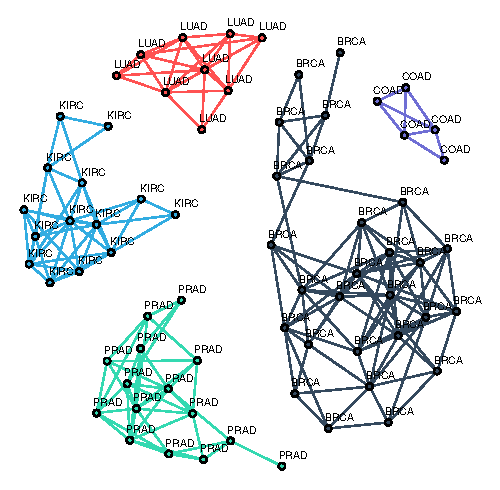
\includegraphics[width=.475\textwidth]{cancer-rna/latex/figures/cancer-rna-graph-subset.eps}
  \caption{Clustering the cancer tumor type \textsf{PANCAN} dataset with \textsf{SGL}$(K = 10, \beta = 5)$.}
  \label{fig:cancer-gene-sgl}
\end{figure}
